\subsection{Implementierung der Datenbank}
\label{subsec:implementierung-der-datenbank}

In diesem Unterkapitel werden die Einbindung der Datenbank in die Applikation sowie die Implementierung grob erläutert.
Der Hauptfokus liegt hierbei auf der Einbindung und der Methode zum Erstellen über Flask-SQLAlchemy.
Die Datenbank wurde mithilfe der Bibliothek Flask-SQLAlchemy erstellt.
Hierbei wurde die Bibliothek Flask-Migration für die Verwaltung von Datenbankschemata genutzt.

SQLAlchemy stellt \ac{ORM} bereit, mit welchem die relationalen Datenbanktabellen als objektorienhtierte Python-Klassen
dargestellt werden können.
Dardurch konnte die in \ref{subsec:datenbankdesign-und-strukturkonzeption} dargestellte Datenbankstruktur, ohnen die aktive Nutzung von SQL-Befehlen definiert und umgesetzt werden.
Hierbei enspricht jede Klassen einer der Tabellen.
Die Attribute der Klassen bilden die Spalten der Tatellen ab, die Fremdschlüssel zwischen den Tabellen werden über Relationship-Objekte beschrieben.
Die Klassen werden im Ordner \code{models} definiert.
Zur Veranschaulgung wird der Aufbau an dem Beispiel der Tabelle bzw. der Klasse \code{Report_Table} aus der Datei \code{report.py} kurz erläutert, siehe Abblidung \ref{fig: Beispiel der Tabelle-Klasse Report_Table}.

\begin{figure}[H]
    \centering
    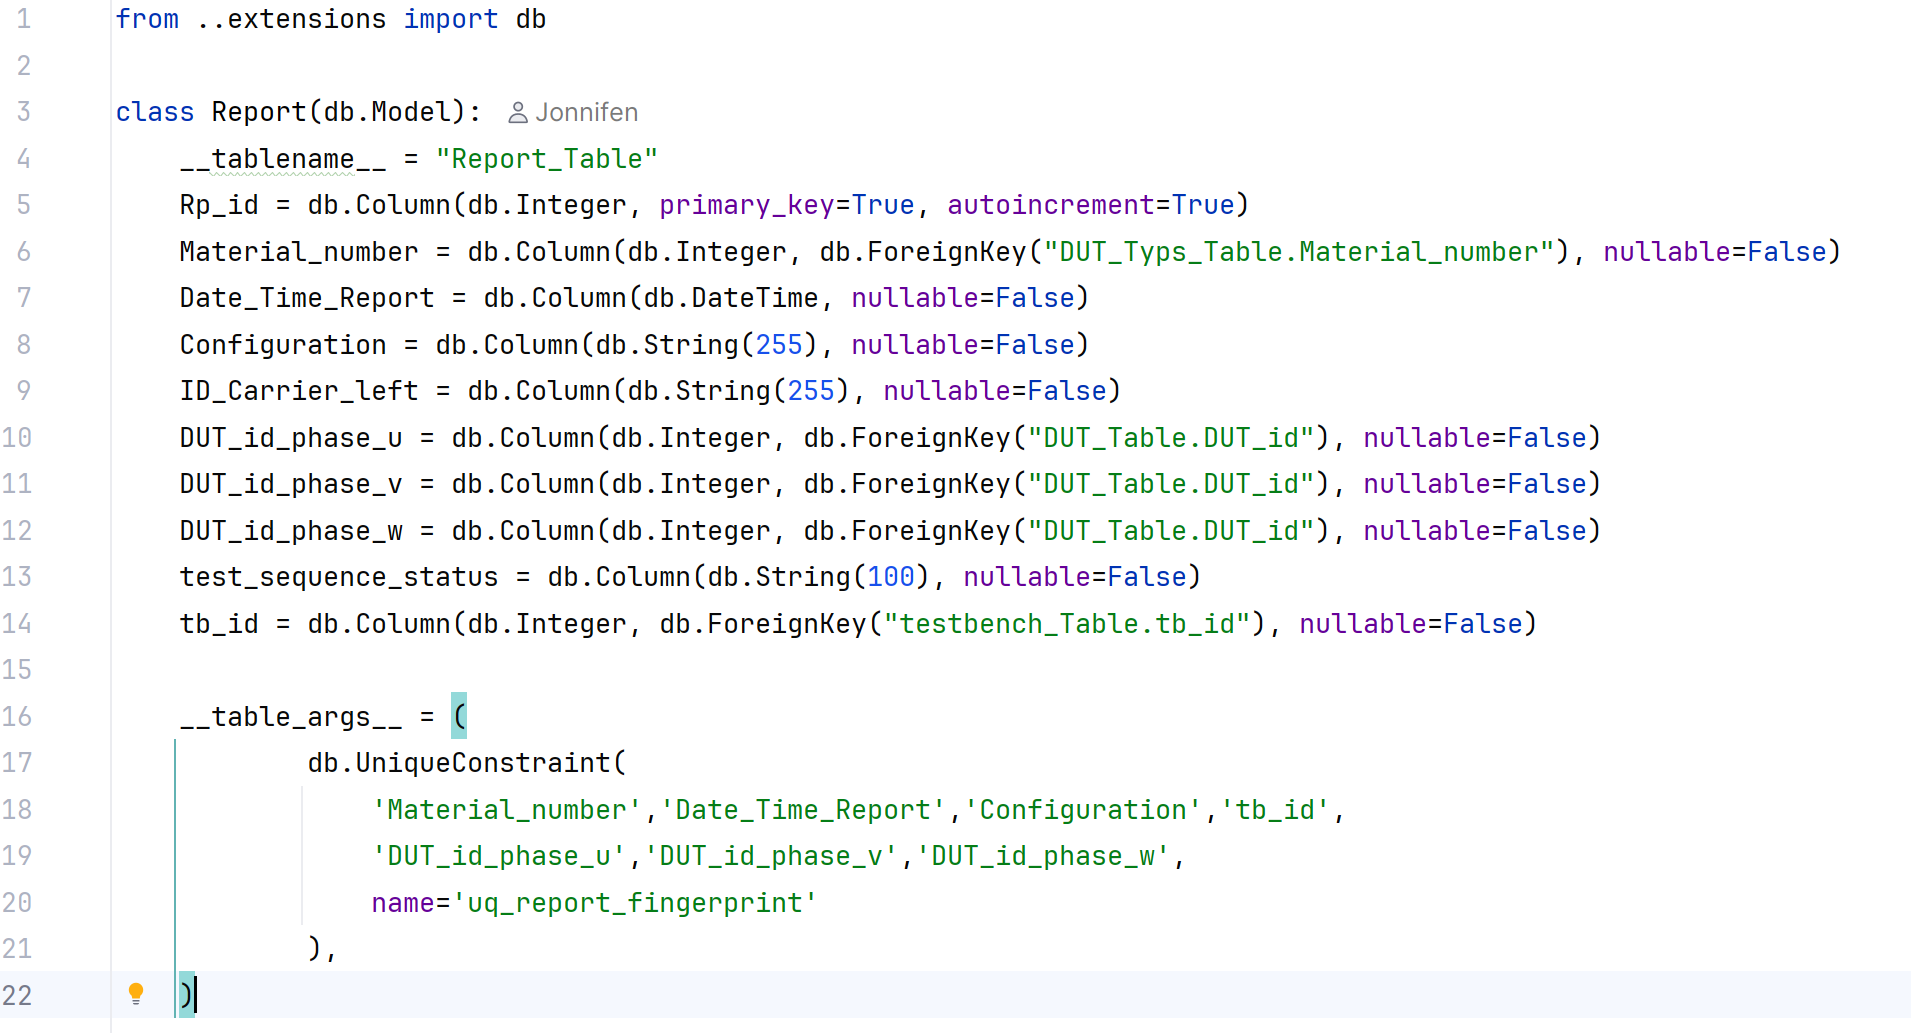
\includegraphics[width=1\textwidth]{Grafiken/5.4 Class.png}
    \caption{Beispiel der Tabelle-Klasse Report_Table}
    \label{fig: Beispiel der Tabelle-Klasse Report_Table}
    {Quelle: Eigene Darstellung}
\end{figure}



Alle Klassen aus \code{models} sind identisch aufgebau und folgen dem gleichem Schema.
Sie besitzen alle den Import der globalen Instants \code{db} aus dem Module \code{extensions}.
Diese Instands bindent SQLAlechemy in die Flask-Applikation ein und wird bei starten der Hauptapplikation initialisiert.
Über diese Instanz \code{db} können alle Modelle registriert und Datenbankoperationen wie Abfragen, Einfügungen oder Aktualisierungen ausgeführt werden.
Die Funktion zum erstellen Hauptapplikation ist in Abblidung \ref{fig: Funktion für das Erstellen der Hauptapplikation} dargestellt, sie liegt in der Datei \code{__init__.py} und wird über \code{run.py} ausgeführt.

\begin{figure}[H]
    \centering
    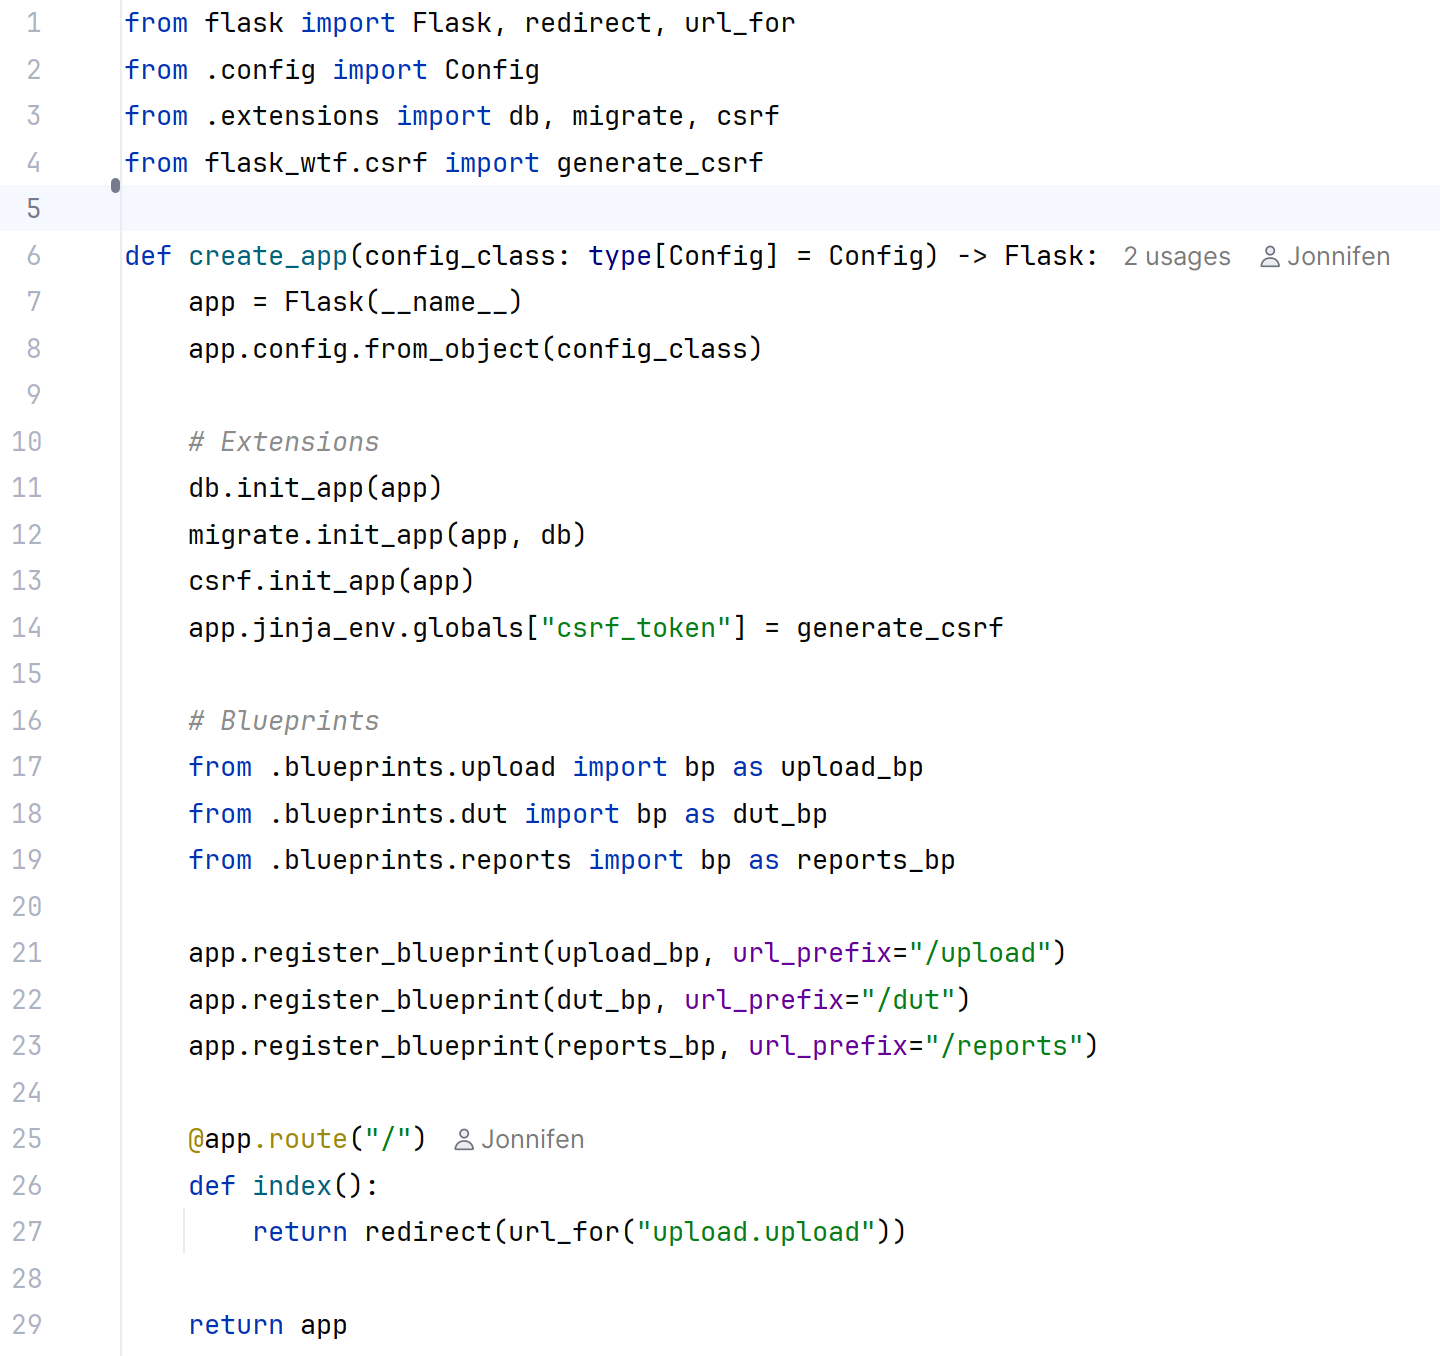
\includegraphics[width=1\textwidth]{Grafiken/createapp.png}
    \caption{Funktion für das Erstellen der Hauptapplikation}
    \label{fig: Funktion für das Erstellen der Hauptapplikation}
    {Quelle: Eigene Darstellung}
\end{figure}

Die Metadaten \code{__tablename__} in Abblidung \ref{fig: Beispiel der Tabelle-Klasse Report_Table} legen fest, wie die Tabelle in der Datenbank heißen soll.
In Zeile 5 bis 14 werden die Attribute bzw. Tabellen Spalte definieriert.
Am ende der Klasse wird ein Table Constraints über \code{__table_args__} defineirt welche als Datenbankseitiger Dupplizierungsschutz bind.
Dieser sorgt dafür, dass derselbe XML-Bericht versehentlich mehrfach importiert wird.
Es könen nicht zwei Datensätze mit denselben Werten existieren.
Dies dient als zusätzliche Sicherheitsinstanz neben den selbst erstellten Dupplizierungsschutz in \code{ingest\_xml()}.





